\subsection{Wat is een taal?}

\vspace{0.5cm}

\begin{theo}[String over een alfabet $\Sigma$]{String over een alfabet Sigma}
    Een \textbf{string} over een alfabet $\Sigma$ is een eindige opeenvolging van nul, één of meer elementen van $\Sigma$.
\end{theo}

\begin{theo}[Taal $L$ over een alfabet $\Sigma$]{Taal L over een alfabet Sigma}
    Een \textbf{taal} $L$ over een alfabet $\Sigma$ is een verzameling van strings over $\Sigma$.
\end{theo}

\subsection{Een algebra van talen}

\vspace{0.5cm}

\begin{theo}[Een algebra- of algebraïsche structuur]{Een algebra- of algebraïsche structuur}
    Een algebra- of algebraïsche structuur is een verzameling met daarop een aantal inwendige operaties:
    dikwijls binaire operaties, maar unair of met grotere ariteit kan ook. Zo wordt de verzameling van
    alle talen over een alfabet $\Sigma$ een algebra als we als operaties unie, doorsnede, complement, etc.\ definïeren.
    Meer concreet: als $L_1$ en $L_2$ twee talen zijn, dan is
    \begin{itemize}
        \item de unie ervan een taal: $L_1 \cup L_2$
        \item de doorsnede ervan een taal: $L_1 \cap L_2$
        \item het complement ervan een taal: $\overline{L_1}$
    \end{itemize}
\end{theo}

\begin{pro}[Concatenatie van twee talen]{Concatenatie van twee talen}
    Gegeven twee talen $L_1$ en $L_2$ over hetzelfde alfabet $\Sigma$, dan noteren we de concatenatie van
    $L_1$ en $L_2$ als $L_1L_2$ en definïeren we:
    \begin{equation*}
        L_{1}L_{2} = \{ xy  \ | \ x \in L_1,  \ y \in L_2\}
    \end{equation*}
    \vspace{-0.3cm}
\end{pro}

\begin{pro}[De Kleene ster van een taal]{De Kleene ster van een taa}
    De Kleene ster van een taal wordt gedefinieerd als volgt:
    \begin{equation*}
        L^* = \cup_{n \geq 0}L^n
    \end{equation*}
    \vspace{-0.5cm}
\end{pro}

\newpage

\subsection{Reguliere expressies en reguliere talen}

\vspace{0.5cm}

\begin{theo}[Reguliere Expressie (RE) over een alfabet $\Sigma$]{Reguliere Expressie (RE) over een alfabet Sigma}
    E is een \textbf{reguliere expressie} over een alfabet $\Sigma$ indien E van de vorm is
    \begin{itemize}
        \item $\epsilon$
        \item $\phi$
        \item $a$ waarbij $a \in \Sigma$
        \item ($E_{1}E_{2}$) waarbij $E_1$ en $E_2$ reguliere expressies zijn over $\Sigma$
        \item ($E_{1}^*$) waarbij $E_1$ een reguliere expressies is over $\Sigma$
        \item ($E_{1}|E_{2}$) waarbij $E_1$ en $E_2$ reguliere expressies zijn over $\Sigma$
    \end{itemize}
    \vspace{-0.3cm}
\end{theo}

\begin{theo}[Reguliere taal]{Reguliere taal}
    Een reguliere expressie $E$ bepaalt een \textbf{reguliere taal} $L_E$ over hetzelfde alfabet $\Sigma$ als volgt:
    \begin{itemize}
        \item als $E = a \ (\text{met} \ a \in \Sigma)$ dan is $L_E = \{a\}$
        \item als $E = \epsilon$ dan is $L_E = \{\epsilon\}$
        \item als $E = \phi$ dan is $L_E = \emptyset$
        \item als $E = (E_{1}E_{2})$ dan $L_E = L_{E_1}L_{E_2}$
        \item als $E = {(E_{1})}^{*}$ dan $L_E = L_{E_1}^*$
        \item als $E = (E_{1}|E_{2})$ dan $L_E = L_{E_1} \cup L_{E_2}$
    \end{itemize}
    \vspace{-0.3cm}
\end{theo}

\subsection{Eindge toestandsautomaten}

\vspace{0.5cm}

\begin{theo}[Niet-deterministische eindige toestandsautomaat (NFA)]{Niet-deterministische eindige toestandsautomaat}
    Een \textbf{niet-deterministische eindige toestandsautomaat} is een 5-tal $(Q,\Sigma, \delta, q_s, F)$ waarbij

    \vspace{0.5cm}

    \begin{minipage}{.56\textwidth}
        \begin{itemize}
            \item $Q$ een eindige verzameling toestanden is
            \item $\Sigma$ is een eindig alfabet
            \item $\delta$ is de overgangsrelatie van de automaat
            \item $q_s$ is de starttoestand
            \item $F \subset Q$ is de verzameling eindtoestanden
        \end{itemize}
    \end{minipage}
    \begin{minipage}{.4\textwidth}
        \begin{center}
            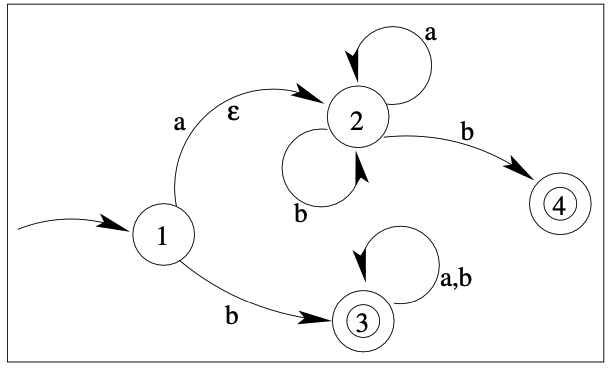
\includegraphics[scale = 0.25]{Images/NFA}
        \end{center}
    \end{minipage}
\end{theo}

\newpage

\begin{theo}[Een string $s$ wordt aanvaard door een NFA]{Een string s wordt aanvaard door een NFA}
    Een string $s$ wordt aanvaard door een NFA $(Q,\Sigma, \delta, q_s, F)$ indien
    er een sequentie $q_s = q_0 \overset{a_0}{\to} \ldots \overset{a_{n-1}}{\to} q_n$
    van overgangen bestaat met $q_n \in F$ zodat s de $\epsilon$-compressie, wat bekomen wordt door
    in $\epsilon$ te schrappen in de string, is van $a_0 \ldots a_{n-1}$. \\
    
    \noindent \textbf{Dus:} Voor toestanden $p$,$q$ en string $w \in \Sigma^*$ schrijven we $p \overset{w}{\rightsquigarrow} q$
    indien er een sequentie van overangen $ p \overset{a_0}{\to} \ldots \overset{a_{n-1}}{\to} q$ bestaat zodat $w$
    de $\epsilon$-comprssie is van $a_0 \ldots a_{n-1}$.
\end{theo}

\begin{theo}[De taal door een NFA $M$ bepaald]{De taal door een NFA M bepaald}
    Een taal $L$ wordt bepaald door een NFA $M$, indien $L$ de verzameling van strings is die $M$ aanvaardt.
    We noteren de taal van $M$ als $L_M$.
\end{theo}

\begin{theo}[Equivalentie van twee NFA's]{Equivalentie van twee NFA's}
    Twee NFA's worden \textbf{equivalent} genoemd als ze dezelfde taal bepalen.
\end{theo}

\subsection{De algebra van NFA's}

\vspace{0.5cm}

\begin{pro}[De unie van twee NFA's]{De unie van twee NFA's}
    \underline{Gegeven}: ${NFA}_1 = (Q_1,\Sigma, \delta_1, q_{s_1}, \{q_{f_1}\})$ en ${NFA}_2 = (Q_2,\Sigma, \delta_2, q_{s_2}, \{q_{f_2}\})$ \\

    \begin{minipage}{.63\textwidth}
        De unie ${NFA}_1 \cup {NFA}_2$ is de $NFA = (Q,\Sigma, \delta, q_s, F)$ waarbij

        \begin{itemize}
            \item $Q = Q_1 \cup Q_2 \cup \{ q_s, q_f \}$
            \item $F = \{q_f\}$
            \item $\delta$ is gedefnieerd als:
            \begin{itemize}
                \item $\forall q \in Q_{i} \backslash \{q_{f_{i}}\}, \ x \in \Sigma_{\epsilon}, \ i = 1,2: \ \delta(q,x) = \delta_i(q,x)$
                \item $\delta(q_s, \epsilon) = \{q_{s_{1}}, q_{s_{2}}\}$
                \item $\forall x \in \Sigma: \delta(q_s, x) = \emptyset$
                \item $i = 1,2: \delta(q_{f_{i}}, \epsilon) = \{q_f\}$
                \item $\forall x \in \Sigma, i = 1,2: \delta(q_{f_{i}}, x) = \emptyset$
            \end{itemize}
        \end{itemize}
    \end{minipage}
    \begin{minipage}{.33\textwidth}
        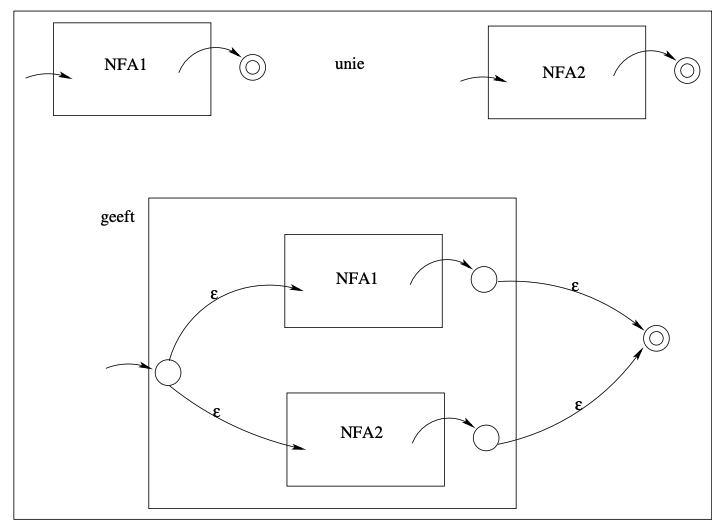
\includegraphics[scale = 0.225]{Images/UnieNFA}
    \end{minipage}
\end{pro}

\newpage

\begin{pro}[De concatenatie van twee NFA's]{De concatenatie van twee NFA's}
    \begin{center}
        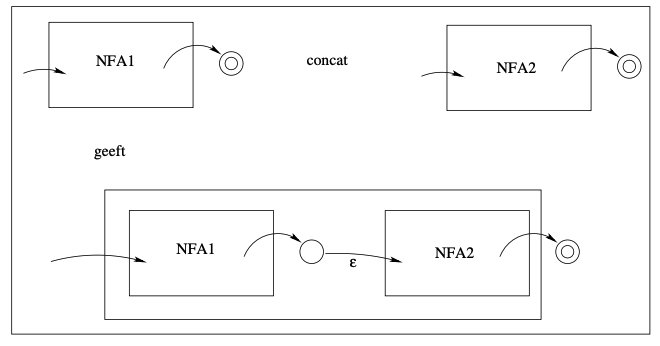
\includegraphics[scale = 0.35]{Images/ConcatNFA}
    \end{center}
\end{pro}

\begin{pro}[De ster van een NFA]{De ster van een NFA}
    \begin{center}
        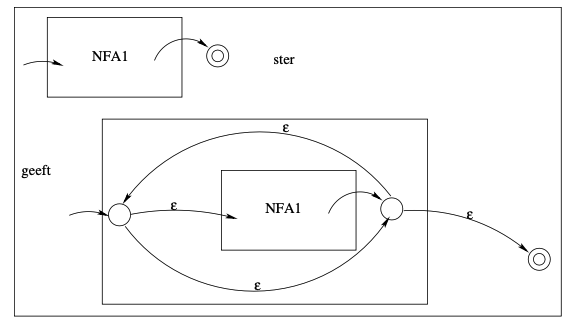
\includegraphics[scale = 0.4]{Images/SterNFA}
    \end{center}
\end{pro}

\subsection{Van RE naar NFA}

\vspace{0.5cm}

\begin{theo}[Van RE naar NFA]{Van RE naar NFA}
    We hebben alle ingrediënten om van een reguliere expressie RE een NFA te maken, en zodanig dat de $L_{RE} = L_{NFA}$.
    Vermits reguliere expressies inductief gedefinieerd zijn zullen we voor elk lijntje van die definitie een overeenkomstige NFA definiëren.
    De drie basisgevallen, namelijk $\epsilon$, $\phi$ en $a \in \Sigma$, zijn triviaal te modeleren als NFA.
    De drie recursieve gevallen beschrijven we als volgt: laat $E_{1}$ en $E_{2}$ twee reguliere expressies zijn, dan is
    \begin{itemize}
        \item $NFA_{E_{1}E_{2}} = \text{concat}(NFA_{E_{1}},NFA_{E_{2}})$
        \item $NFA_{E_{1}^{*}} = \text{ster}(NFA_{E_{1}})$
        \item $NFA_{E_{1}|E_{2}} = \text{unie}(NFA_{E_{1}},NFA_{E_{2}})$
    \end{itemize}
    \noindent De constructie hierboven bewaart de taal, t.t.z. $L_{NFA_{E}} = L_{E}$.
\end{theo}

\subsection{Van NFA naar RE}

\vspace{0.5cm}

\begin{theo}[GNFA]{GNFA}
    Een \textbf{GNFA} is een eindige toestandsmachine met de volgende wijzigingen en beperkingen: \\

    % \begin{itemize}
    %     \item er is slechts één eindtoestand en die is verschillend van de starttoestand
    %     \item vanuit de starttoestand vertrekt er juist één boog naar elke andere toestand; er komen geen bogen aan in de starttoestand
    %     \item in de eindtoestand komt juist één boog aan vanuit elke andere toestand; uit de eindtoestand vertrekken geen bogen
    %     \item voor paar \(p\),\(q\) (let op: p = q is geldig) van andere toestanden (geen start- of eindtoestand) is er juist één boog van \(p \to q\) en één boog van \(q \to p\).
    %     \item  de bogen hebben als label een reguliere expressie
    % \end{itemize} 
    \begin{minipage}{.56\textwidth}
        \begin{itemize}
            \item er is slechts één eindtoestand en die is verschillend van de starttoestand
            \item vanuit de starttoestand vertrekt er juist één boog naar elke andere toestand; er komen geen bogen aan in de starttoestand
            \item in de eindtoestand komt juist één boog aan vanuit elke andere toestand; uit de eindtoestand vertrekken geen bogen
            \item voor paar \(p\),\(q\) (let op: \(p\) = \(q\) is geldig) van andere toestanden (geen start- of eindtoestand) is er juist één boog \(p \to q\) en één boog \(q \to p\).
            \item  de bogen hebben als label een reguliere expressie
        \end{itemize} 
    \end{minipage}
    \begin{minipage}{.4\textwidth}
        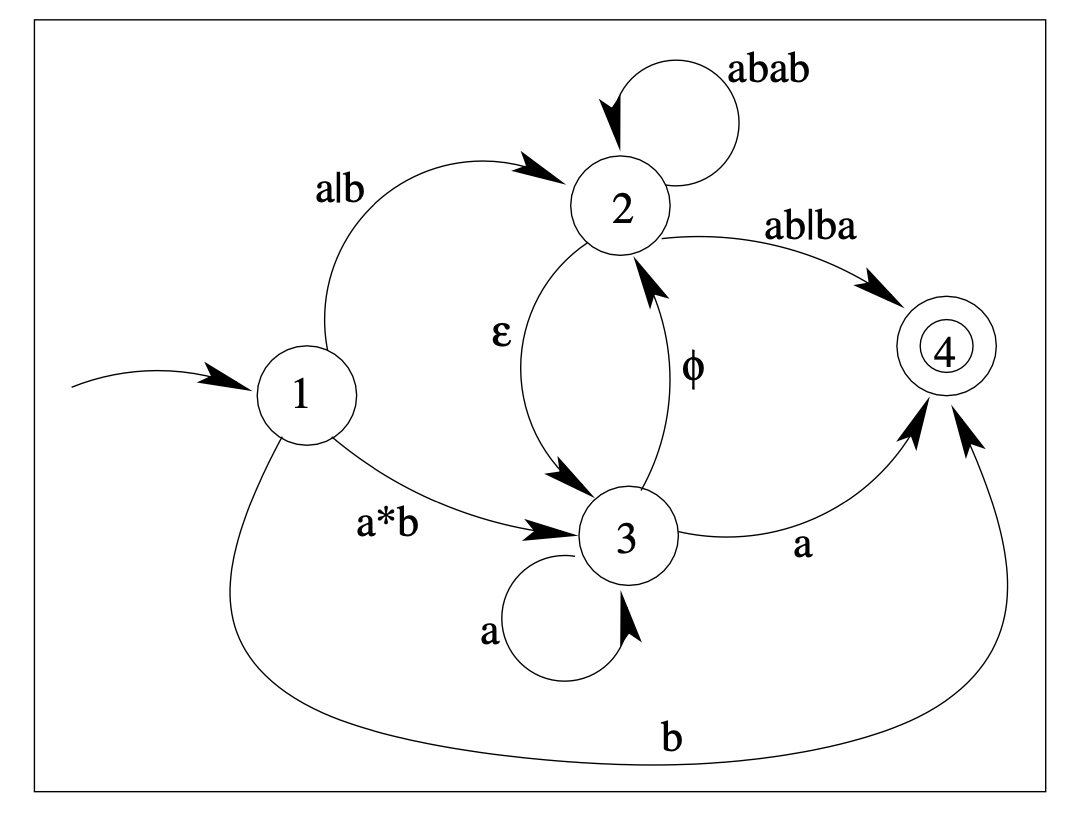
\includegraphics[scale = 0.35]{Images/GNFA.png}
    \end{minipage}
\end{theo}

\begin{alg}[NFA $\to$ RE]{NFA naar RE}
    \begin{enumerate}
        \item Maak van de NFA een GNFA
        \begin{itemize}
            \item Behoud alle toestanden en bogen van de NFA
            \item Als er meerdere bogen zijn tussen twee toestanden gelabeld met symbolen \(a_{1} \ldots a_{n} \) vervang deze door één boog met als label \(a_{1} | \ldots | a_{n} \)
            \item Voer een nieuwe starttoestand in en een \(\epsilon\)-boog naar de oude starttoestand
            \item Voer een nieuwe eindtoestand in en \(\epsilon\)-bogen vanuit elke oude eindtoestand
            \item Voor elke boog die ontbreekt tussen twee toestanden om een GNFA te bekomen, voer een \(\phi\)-boog in
        \end{itemize}
        \item Reduceer de GNFA: \vspace{0.3cm} \\
            \begin{minipage}{.453\textwidth} 
                Kies een willekeurige toestand \(X\) verschillend van de start- of eindtoestand, ga naar stap 3 als dit niet mogelijk is.
                Voor elk paar toestanden \(A\) en \(B\) (let op: \(A\) = \(B\) is geldig) verschillend van X bevat de GNFA een unieke boog \(A \to B\) met label \(E_{4}\), 
                \(A \to X\) met label \(E_{1}\), \(X \to X\) met label \(E_{2}\) en \(X \to B\) met label \(E_{3}\). Vervang het label op de boog \(A \to B\) door \(E_{4} | E_{1}E_{2}^{*}E_{3}\).
                Doe dit voor alle keuzes voor A en B. Verwijder daana de knoop X en herhaal.
            \end{minipage}
            \begin{minipage}{.43\textwidth}
                \hspace{0.3cm}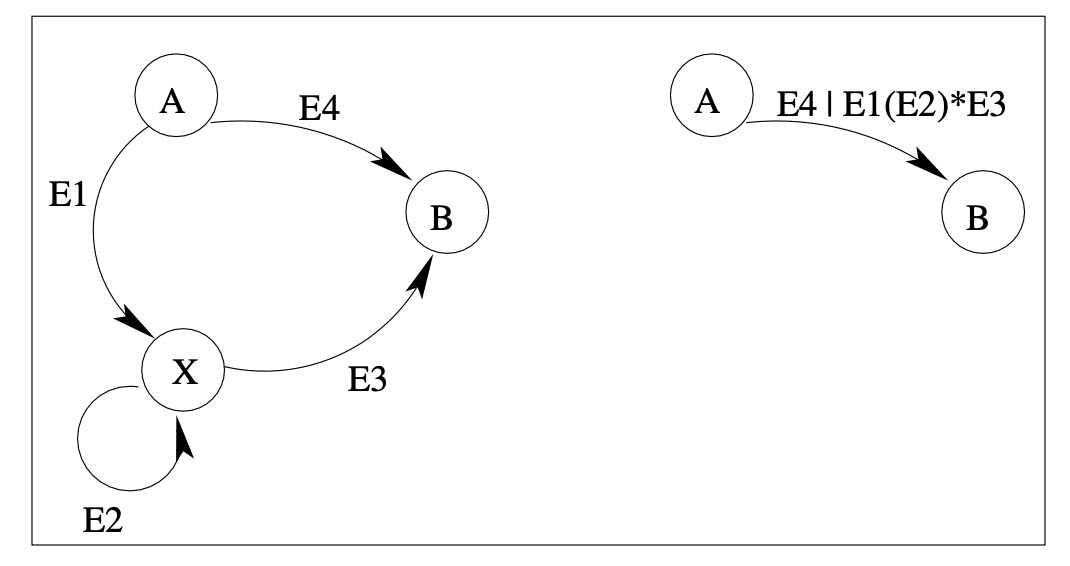
\includegraphics[scale = 0.375]{Images/GNFAToestandVerwijderen}
            \end{minipage}
        \item Bepaal RE: de boog van de GNFA heeft als label de gezochte RE
    \end{enumerate}
\end{alg}

\newpage

\subsection{Deterministische eindige toestandsmachines}

\vspace{0.5cm}

\begin{theo}[Deterministische eindige toestandsmachines]{Deterministische eindige toestandsmachines}
    Een NFA is een DFA indien \(\delta\) geen \(\epsilon\)-overgangen bevat en 
    indien voor elke \(p \in Q\) en elke \(a \in \Sigma\) een unieke \(q \in Q\) 
    bestaat zodat \(p \overset{a}{\to} q\). Het komt erop neer dat in een DFA, \(\delta\) 
    een totale functie $Q \times \Sigma \to Q$ is. Voor DFA's zullen a
    we de unieke toestand q zodat \(p \overset{a}{\to} q\) dan ook noteren als \(\delta(p,a)\).
\end{theo}

\begin{pro}[Doorsnede, verschil en complement van DFA's]{Doorsnede, verschil en complement van DFA's}
    \underline{Gegeven}: ${\text{DFA}}_1 = (Q_1,\Sigma, \delta_1, q_{s_1}, \{q_{f_1}\})$ en ${\text{DFA}}_2 = (Q_2,\Sigma, \delta_2, q_{s_2}, \{q_{f_2}\})$ \\

    We maken een generische pdoruct DFA $(Q,\Sigma, \delta, q_s, F)$ als volgt:
    \begin{itemize}
        \item $Q = Q_1 \times Q_2$
        \item $\delta(p \times q, x) = \delta_1(p,x) \times \delta_2(q,x)$
        \item $q_s = (q_{s_1},q_{s_2})$
        \item 
            Om tot een volledig definitie te komen, moeten we nog $F$ bepalen:
            \begin{itemize}
                \item $F = F_1 \times F_2$: de DFA is de doorsnede van de twee talen
                \item $F = (F_1 \times Q_2) \cup (Q_1 \times F_2)$: de DFA is nu de unie van de twee talen
                \item $\forall i \neq j \in [1,2]: \ F =  F_i \times (Q_j \times F_j)$: de DFA bepaalt nu de strings die tot $L_i$ behoren, maar niet tot $L_j$
                \item $F = (Q_1 \backslash F_1) \times (Q_2 \backslash F_2)$: de DFA bepaalt nu de strings die tot geen van beide talen behoren.
            \end{itemize}
    \end{itemize}
    Hieruit volgt ook dat de unie, doorsnede en complement van twee reguliere talen ook regulier zijn. Daaruit volgt ook dat het
    complement van een reguliere taal ook regulier is, want $\overline{L} = \Sigma^* \backslash L$.
\end{pro}

\begin{lem}[DFA en NFA equivalentie]{DFA en NFA equivalentie}
    Elke NFA is equivalent met een DFA, m$.$a$.$w$.$ we kunnen elke NFA \((Q, \Sigma, \delta, q_s, F)\) herleiden tot een
    equivalente DFA \((Q', \Sigma, \delta', q_s', F')\) waarbij
    \begin{itemize}
        \item \(Q'\): de verzameling van alle deelverzamelingen $q'$ van $Q$ die gesloten zijn onder \(\epsilon\)-bogen, dus
              \(p \in q' \ \wedge \ p \overset{\epsilon}{\to} q \ \Rightarrow \ q \in q'\)
        \item \(\delta': Q' \times \Sigma \rightarrow Q'\)
        \item \(q_{s}' = \{q_s,q \ | \ q_s \overset{\epsilon}{\rightsquigarrow} q \}\)
        \item \(F' = \{q' \in Q' \ | \ q' \cap F \neq \emptyset \}\)
    \end{itemize}
    \vspace{-0.3cm}
\end{lem}

\newpage

\begin{prf}[DFA en NFA equivalentie]{prf - DFA en NFA equivalentie}
    Uit constructie volgt dat de geconstrueerde automaat \((Q', \Sigma, \delta', q_s', F')\) een DFA is.
    Wat betreft equivalentie, moeten we verifiëren dat \(\forall w \in \Sigma^*:  q_s \overset{w}{\rightsquigarrow} F \Leftrightarrow q_s' \overset{w}{\rightsquigarrow} F'\). 
    De essentie van dat bewijs is dat voor elke \(w \in \Sigma^*\), als in de DFA geldt dat \(q_s' \overset{w}{\rightsquigarrow} q\) (in de DFA) dan is \(q\ = q_w = \{ q \ | \ q_s \overset{w}{\rightsquigarrow} q \}\) (in de NFA).
    Dit is eenvoudig inductief te bewijzen gebruik makend van het feit dat \(q' = q_w' \Rightarrow \delta'(q',a) = q_{wa}'\). Dan geldt dat de 
    DFA een string $w$ aanvaardt als voor de unieke toestand \(q'\) zodat \(q_s' \overset{w}{\rightsquigarrow} q'\) geldt dat \(q' \cap F \neq \emptyset \ \Leftrightarrow \ q_w' \cap F \neq \emptyset \ \Leftrightarrow\) de NFA aanvaardt w.
\end{prf}

\begin{theo}[$f$-string]{f-string}
    We noemen een string $s$ een $f$-string vanuit $q$ van de DFA indien \(\delta^*(q,s) \in F\), t$.$t$.$z$.$ indien er een pad is van $q$ naar een toestand van $F$ die s genereert. $F$-gelijke toestanden
    zijn dan toestanden met dezelfde $f$-strings. \vspace{0.3cm}\\
    \textbf{Opmerking:} \(q \in F \Leftrightarrow \epsilon \text{ is een $f$-string vanuit $q$}\)
\end{theo}

\begin{theo}[$f$-gelijk]{f-gelijk}
    Twee toestanden \(q_1,q_2\) zijn $f$-gelijk indien
    \begin{equation*}
        \{ s \in \Sigma^* \ | \ \delta^*(q_1,s) \in F\} = \{s \in \Sigma^* \ | \ \delta^*(q_2,s) \in F\}
    \end{equation*}
    In woorden, als $q_1$ en $q_2$ exact dezelfde $f$-strings hebben.
\end{theo}

\begin{pro}[$f$-gelijk]{pro - f-gelijk}
    \begin{itemize}
        \item De relatie $f$-gelijk is een equivalentie-relatie.
        \item Als $p,q$ $f$-gelijk zijn dan geldt voor elk symbool $a$ dat \(\delta(p,a)\) en \(\delta(q,a)\) ook $f$-gelijk zijn.
        \item Als $p,q$ $f$-gelijk zijn dan geldt \(p \in F \Leftrightarrow q \in F\).
    \end{itemize}
\end{pro}

\begin{prf}[Eigenschappen van de $f$-gelijk relatie]{prf - Eigenschappen van de f-gelijk relatie}
    \begin{itemize}
        \item Het is triviaal om te bewijzen dat $f$-gelijkheid een equivalentie-relatie is. Dit kan je doen door de reflexiviteit, symmetrie en transitiviteit van de relatie na te gaan.
        \item Veronderstel dat $p,q$ $f$-gelijk zijn en veronderstel voor een willekeurig symbool $a$ dat \(\delta(p,a) = p', \delta(q,a) = q'\). De $f$-strings van $p$ en $q$ zijn gelijk,
              en dus ook hun $f$-strings van de vorm $as$. De $f$-strings van $p'$ zijn de strings $s$ zodat $as$ een $f$-string is van $p$.
              Hetzelfde geldt voor $q'$. Bijgevolg hebben $p',q'$ dezelfde $f$-strings en zijn ze dus $f$-gelijk.
        \item Als $p$ en $q$ $f$-gelijk zijn, en $p \in F$ dan is $\epsilon$ een $f$-string van $p$ en dus ook van $q$. Aangezien er in een DFA geen $\epsilon$-bogen zijn, is $q \in F$.
              Hetzelfde geldt in de andere richting. 
    \end{itemize}
    \vspace{-0.5cm}
\end{prf}

\newpage

\begin{theo}[Minimale DFA]{Minimale DFA}
    Een DFA is minimaal als er geen enkele andere DFA bestaat die dezelfde taal bepaalt en minder toestanden heeft, m$.$a$.$w$.$ 
    DFA$_{\text{min}}$ is een DFA, equivalent met DFA, en alle toestanden zijn $f$-verschillend.
    \vspace{-0.3cm}
\end{theo}

\begin{lem}[DFA$_{\text{min}}$]{minDFA}
    \begin{itemize}
        \item DFA$_{\text{min}}$ is een DFA, equivalent met DFA, en alle toestanden zijn $f$-verschillend.
        \item Als een DFA $N$ = $(Q_1,\Sigma, \delta_1, q_s, F_1)$  een DFA is zonder onbereikbare toestanden en waarin elke twee toestanden $f$-verschillend zijn, 
        dan bestaat er geen machine met strikt minder toestanden die dezelfde taal bepaalt.
    \end{itemize}
\end{lem}

\begin{prf}[DFA$_{\text{min}}$]{prf - minDFA}
    \begin{itemize}
        \item 
        DFA$_min$ is een DFA omdat $f$-gelijkheid van toestanden $p$ en $q$ de $f$-gelijkheid van \(\delta(p,a)\) en \(\delta(q,a)\) impliceert. Het gevolg is dat verschillende bogen met hetzelfde symbool
        vanuit $f$-gelijke $p$ en $q$ versmelten. Om aan te tonen dat DFA en DFA$_{\text{min}}$ equivalent zijn, is de essentiële eigenschap dat elke equivalentie-klasse $Q_i$ en elk element \(p \in Q_i\)
        dezelfde $f$-strings heeft. Dus heeft $\tilde{q}_s$ dezelfde $f$-strings als $q_s$, en deze verzameling is dus de taal die beide DFA's bepalen. Aantonen dat een string $w$ een $f$-string is van $Q_i$
        als en slechts als $w$ een $f$-string is van \(q \in Q_i\) gebeurt door inductie op de lengte van $w$, gebruikmakend van het feit dat voor elke \(Q_i,Q_j\)
        \begin{equation*}
            p \in Q_i, \ q \in Q_j, \ \forall a \in \Sigma: \ Q_i \overset{a}{\to} Q_j \ \Leftrightarrow \ p \overset{a}{\to} q 
        \end{equation*}
        Tenslotte, twee verschillende toestanden $Q_i, Q_j$ bevatten $f$-verschillende toestanden. Aangezien de $f$-strings van $Q_i$ en $Q_j$ die van hun elementen zijn, zijn ze $f$-verschillend.
        \item    
        Veronderstel dat \(Q_1 = \{q_s,q_1, \ldots, q_n\}\) waarbij \(q_s\) de starttoestand is. 
        Stel dat \(N_2 = (Q_2,\Sigma, \delta_2, q_s, F_2)\) een DFA is met minder toestanden dan $N$.
        Vermits in $N$ elke toestand bereikbaar is, bestaan er strings \(\forall i \in \mathbb{N}_0^+: s_i\) zodanig dat \(\delta_1^*(q_s,s_i) = q_i\). 
        Vermits \(N_2\) minder toestanden heeft moet voor een \(i \neq j: \delta_2^*(p_s,s_i) = \delta_2^*(p_s,s_j)\). Vermits \(q_i\) en \(q_j\)
        $f$-verschillend zijn, is er een string \(s\) zodat \(\delta_1^*(q_i,s) \in F_1\) en \(\delta_1^*(q_j,s) \notin F_1\) of omgekeerd.
        Dus ook \(\delta_1^*(q_s,s_is) \in F_1\) en \(\delta_1^*(q_s,s_js) \notin F_1\) of omgekeerd. Dit betekent dat DFA$_1$ van de strings $s_is$ en $s_js$ er juist één accepteert.
        Maar N$_2$ zal beide strings $s_is$ en $s_js$ accepteren of geen van beiden, aangezien het parsen van $s_i$ en $s_j$ naar dezelfde node leidt, waarna hetzelfde pad gevolgd wordt om $v$ te parsen.
        Dus kunnen de DFA's N en N$_2$ niet dezelfde taal bepalen.
    \end{itemize}
\end{prf}

\newpage

\begin{theo}[DFA isomorfisme]{DFA isomorfisme}
    Een DFA $N_1 = (Q_1, \Sigma, \delta_1, q_{s_1}, F_1)$ is \textbf{isomorf} met een DFA $N_2 = (Q_2, \Sigma, \delta_2, q_{s_2}, F_2)$ als er een bijectie $b: Q_1 \to Q_2$ bestaat zodanig dat
    \begin{itemize}
        \item $b(F_1) = F_2$
        \item $b(q_{s_1}) = q_{s_2}$
        \item $b(\delta_1(q,a)) = \delta_2(b(q),a)$
    \end{itemize}
    Twee isomorfe DFA's bepalen dus dezelfde taal.
\end{theo}

\subsection{Myhill-Nerode relaties op $\Sigma^*$}

\vspace{0.5cm}

\begin{theo}[Fijnheid van partities]{Fijnheid van partities}
    Een partitie $P_1$ is \textbf{fijner} dan een partitie $P_2$ indien
    \begin{equation*}
        \forall x \in P_1,\ \exists y \in P_2: \ x \subseteq y
    \end{equation*}
    Het omgekeerde van fijn is \textbf{grof}.
\end{theo}

\begin{theo}[$\sim_{\text{DFA}}$]{DFAeqklassen}
    Voor een DFA $N = (Q, \Sigma, \delta, q_s, F)$ definiëren we de relatie $\sim_{\text{DFA}}$ op $\Sigma^*$ als volgt:
    \begin{equation*}
        x \sim_{\text{DFA}} y \ \Leftrightarrow \ \delta^*(q_s,x) = \delta^*(q_s,y)
    \end{equation*}
    In woorden: er geldt $x \sim_{\text{DFA}} y$ als en slechts als het parsen van $x$ en $y$ vanuit $q_s$ leidt tot dezelfde toestand $q$, dus $x,y \in \text{reach}(q)$.
\end{theo}

\begin{pro}[$\sim_{\text{DFA}}$]{pro - DFAeqklassen}
    \begin{itemize}
        \item Rechts congruentie van $\sim$: $\forall x,y \in \Sigma^*, \ a \in \Sigma: \ x \sim y \ \Rightarrow \ xa \sim ya $
        \item het aantal equivalentieklassen van $\sim$ is eindig, m$.$a$.$w$.$ $\sim$ heeft een eindige index
        \item $\sim$ verfijnt $\sim_L$, of: $x \sim y \ \Rightarrow \ x \sim_L y$
    \end{itemize}
\end{pro}

\begin{theo}[Myhill-Nerode relatie]{Myhill-Nerode relatie}
    Een equivalentierelatie $\sim$ tussen strings is een \textbf{Myhill-Nerode relatie} voor een taal $L$ als de equivalentieklasse
    voldoet aan bovenstaande eigenschappen. We schrijven: $\sim$ is MN(L)
\end{theo}

\begin{lem}[DFA$_{\sim}^{\text{L}}$]{DFAsimL}
    Gegeven een taal $L$ over $\Sigma$ en een MN(L)-relatie $\sim$ op $\Sigma^*$, dan is DFA$_{\sim}^{\text{L}} = (Q, \Sigma, \delta, q_s, F)$ een DFA die L bepaalt, waarbij
    \begin{itemize}
        \item $Q = \{x_{\sim} \ | \ x \in \Sigma^* \}$
        \item $\delta(x_{\sim},a) = (xa)_{\sim}$
        \item $q_s = \epsilon_{\sim}$
        \item $F = \{x_{\sim} \ | \ x \in L \}$
    \end{itemize}  
    \vspace{-0.3cm}
\end{lem}

\begin{prf}[DFA$_{\sim}^{\text{L}}$]{prf - DFAsimL}
    Dat $\delta$ goed gedefinieerd is, kan je bewijzen door gebruik te maken van de rechtse congruentie van $\sim$.
    Verder zijn alle ingrediënten van de DFA duidelijk, in het bijzonder ook dat $Q$ slechts een eindig aantal toestanden bevat.
    We moeten nog bewijzen dat $L_{\text{DFA}_{\sim}^{\text{L}}} = L$:
    \begin{equation*}
        x \in L_{\text{DFA}_{\sim}^{\text{L}}} \ \Leftrightarrow \ \delta^*(q_s,x) \in F \ \Leftrightarrow \ x_{\sim} \in F \ \Leftrightarrow \ x \in L
    \end{equation*}
    De middelste overgang bekom je door met inductie op de lengte van de string $x$ te bewijzen dat $\delta^*(\epsilon_{\sim},x) = (x)_{\sim}$.
\end{prf}

\begin{lem}[$\sim_{\text{DFA}}$ en $\sim$ zijn elkaars inverse]{simDFA en sim zijn elkaars inverse}
    Voor elke taal $L$ geldt dat de functie die DFA's van $L$ afbeeldt op de de overeenkomstige MN(L)-relatie $\sim_{\text{DFA}}$ en de functie 
    die MN(L)-relaties $\sim$ afbeeldt op de overeenkomstige DFA$_{\sim}^{\text{L}}$, elkaars inversen zijn op een DFA-isomorfisme na.
\end{lem}

% \begin{prf}[$\sim_{\text{DFA}}$ en $\sim$ zijn elkaars inverse]{simDFA en sim zijn elkaars inverse}
% \end{prf}

\begin{lem}[Infimumrelatie van Myhill-Nerode relaties]{Infimumrelatie van Myhill-Nerode relaties}
    Als $E$ een niet lege verzameling van MN(L) relaties is, dan is ook het infimum $\sim_{\text{inf}}$ van $E$ een MN(L)-relatie.
    $\sim_{\text{inf}}$ is de transitieve sluiting van de unie van $E$. Dit betekent dat
    \begin{equation*}
        x \sim_{\text{inf}} y \ \Leftrightarrow \ i \in [0, n-1], \ \sim_i \in E: \ x = x_0 \sim_0 x_1 \sim_1 \ldots \sim_{n-1} x_n = y
    \end{equation*}
    \vspace{-0.5cm}
\end{lem}

\newpage

\begin{prf}[Infimumrelatie van Myhill-Nerode relaties]{prf - Infimumrelatie van Myhill-Nerode relaties}
    We zagen al dat het infimum van een niet lege verzameling $E$ van equivalentierelaties zelf ook een equivalentierelatie is.

    \begin{itemize}
        \item 
            \textbf{Eindigheid:} $\sim_{\text{inf}}$ is een superset van elke willekeurige $\sim \in E$ en heeft dus minder equivalentieklassen
            dan $\sim$. Elke $\sim$ heeft slechts een eindig aantal equivalentieklasse, zodoende ook $\sim_{\text{inf}}$.
        \item 
            \textbf{Rechts congruentie:} Stel $x \sim_{\text{inf}} y$ dan bestaat de sequentie 
            \begin{equation*}
                x = x_0 \sim_0 x_1 \sim_1 \ldots \sim_{n-1} x_n = y
            \end{equation*}
            Aangezien elke $\sim_i$ rechts congruent is, geldt voor elke $a \in \Sigma$ dat 
            \begin{equation*}
                xa = x_0a \sim_0 x_1a \sim_1 \ldots \sim_{n-1} x_na = ya
            \end{equation*}
            Bijgevolg geldt dat $xa \sim_{\text{inf}} ya$ en dus dat $\sim_{\text{inf}}$ rechts congruent is.
        \item 
            \textbf{Verfijnen van $\sim_L$:} Stel $x \sim_{\text{inf}} y$ zodat er een sequentie bestaat 
            \begin{equation*}
                x = x_0 \sim_0 x_1 \sim_1 \ldots \sim_{n-1} x_n = y
            \end{equation*}
            Aangezien elke $\sim_i$ een verfijning is van $\sim_L$, geldt
            \begin{equation*}
                x_0 \in L \Leftrightarrow x_1 \in L \Leftrightarrow \ldots \Leftrightarrow x_n \in L
            \end{equation*}
            We bekomen $x \in L \Leftrightarrow y \in L$ en dus dat $\sim_{\text{inf}}$ een verfijning is van $\sim_L$.
    \end{itemize}
\end{prf}

\begin{pro}[MN(L) toebehorend aan een mininale DFA]{pro - MN(L) toebehorend aan een mininale DFA}
    Het kan nu ook bewezen worden dat de MN(L) relatie die hoort bij de minimale DFA voldoet aan de volgende conditie:
    \begin{equation*}
        x \sim_{\text{inf}} y \ \Leftrightarrow \  \forall s \in \Sigma^*: \ ( xs \in L \Leftrightarrow ys \in L )
    \end{equation*}
    Het is een vorm van $f$-gelijkheid gedefinieerd op strings in plaats van op toestanden.
\end{pro}

\begin{lem}[Stelling van Myhill-Nerode]{Stelling van Myhill-Nerode}
    Laat $L \subseteq \Sigma^*$ een taal zijn over $\Sigma$. De volgende drie uitspraken zijn dan equivalent:
    \begin{itemize}
        \item[$\Leftrightarrow$] $L$ is regulier
        \item[$\Leftrightarrow$] er bestaat een Myhill-Nerode relatie voor $L$
        \item[$\Leftrightarrow$] 
            definieer $\sim$ op $\Sigma^*$ als volgt:
            \begin{equation*}
                x \sim y \ \Leftrightarrow \ \forall s \in \Sigma^*: \ ( xs \in L \Leftrightarrow ys \in L );
            \end{equation*}
            de relatie $\sim$ heeft een eindige index
    \end{itemize}
    \vspace{-0.3cm}
\end{lem}   

\subsection{Pompend lemma voor reguliere talen}

\vspace{0.5cm}

\begin{lem}[Pompend lemma voor reguliere talen]{Pompend lemma voor reguliere talen}
    Voor een reguliere taal $L$ bestaan een pomplengte $d$, zodanig dat als $s \in L$ en $|s| \geq d$, 
    dan bestaat er een verdeling van $s$ in stukken $x$, $y$ en $z$ zodanig dat $s = xyz$ en \\
    \begin{minipage}{0.56\textwidth}
        \begin{itemize}
            \item $\forall i \in \mathbb{N}_0^+: \ xy^iz \in L$
            \item $|y| > 0$
            \item $|xy| \leq d$
        \end{itemize}
    \end{minipage}
    \begin{minipage}{0.4\textwidth}
       \hspace{1.25cm}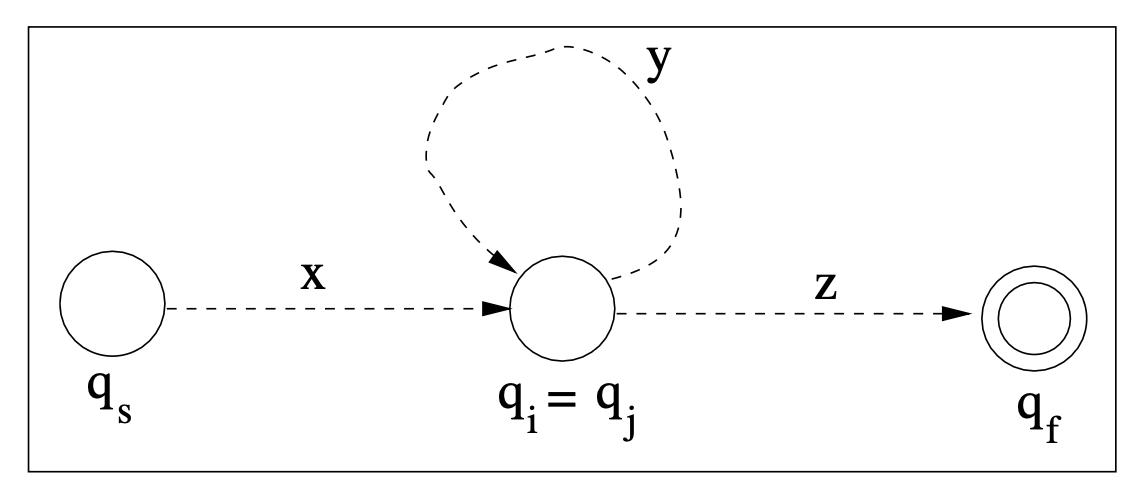
\includegraphics[scale = 0.275]{Images/VerdelingStrings.png}
    \end{minipage}
    \vspace{-0.3cm}
\end{lem}

\begin{prf}[Pompend lemma voor reguliere talen]{prf - Pompend lemma voor reguliere talen}
    Neem een DFA die $L$ bepaalt, neem $d = \#Q$ en neem een willekeurige $s = a_1 \ldots a_n \in L$ met $n \geq d$.
    Beschouw de accepterende sequentie
    \begin{equation*}
        q_s = q_0 \overset{a_1}{\to} q_1 \overset{a_2}{\to} \ldots \overset{a_n}{\to} q_n \in F
    \end{equation*}
    Deze rij van toestanden heeft lengte $n+1$, wat strikt groter is dan $d$. Neem de eerste $d+1$ toestanden van de deze rij,
    dus $q_0,\ldots, q_d$. Er zijn maar $d$ verschillende toestanden, dus er zijn twee gelijke toestanden. 
    Stel dat $q_i = q_j$ met $ 0 \leq i < j \leq d$, dan nemen we $x = a_1 \ldots a_i$, $y = a_{i+1} \ldots a_j$ en $z$ de rest van de string. 
    Alles volgt nu direct, zie desnoods te illustratie in de stelling.
\end{prf}

\subsection{Varianten van eindige toestandsautomaten}

\vspace{0.5cm}

\begin{theo}[Transducer]{Transducer}
    \begin{minipage}{.66\textwidth}
        Een transducer zet een string om in een andere: we passen de definitie van een DFA een beetje aan, zodat ook output kan geproduceerd worden
        De labels zijn nu van de vorm $a/x$ waarbij $a$ in het inputalfabet zit en $x$ in een outputalfabet (inbegrepen de lege string). 
        Wat voor de $/$ staat wordt gebruikt om de weg te vinden in de transducer alsof het een DFA was. Wat na de $/$ staat wordt op de output gezet als die boog genomen wordt. 
        De transducer hiernaast accepteert elke string en geeft als output een 1 voor elke b die vlak na een a komt.
    \end{minipage}
    \begin{minipage}{.3\textwidth}
        \vspace{-0.3cm}\hspace{0.3cm}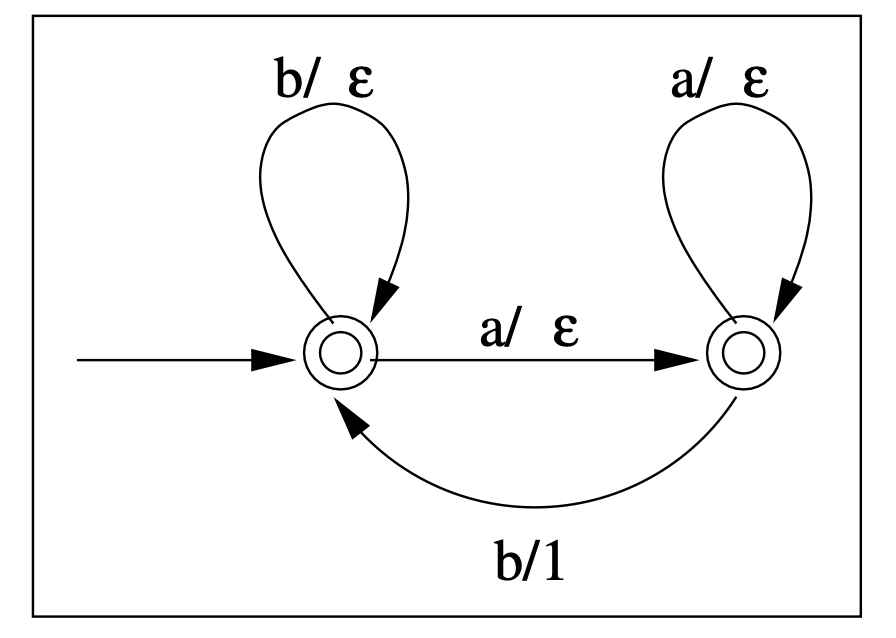
\includegraphics[scale = 0.3]{Images/Transducer.png}
    \end{minipage}
\end{theo}

\newpage

\begin{theo}[Optelchecker]{Optelchecker}
    \begin{minipage}{.75\textwidth}
        Een DFA kan alleen gebruikt worden om te beslissen of een string behoort tot een taal.
        Zo zou je kunnen een taal definiëren van strings die correcte optellingen voorstellen en als die taal regulier is er een DFA voor bouwen.
        Hier is een poging: $\Sigma = \{0,1\}$. De twee getallen  die we willen optellen en het resultaat komen in binair, omgekeerd en we maken ze even lang door bij de kortste(n) wat leidende nullen toe te voegen.
        Dus als we $3$ willen optellen bij $13$, met resultaat $16$, dan hebben we de drie bitstrings $11000$, $10110$ en $00001$. Die mengen we nu systematisch,
        t$.$t$.$z$.$ we maken groepjes van $3$ bits die op de i-de plaats voorkomen en schrijven die groepjes achter elkaar. Dus we hebben 
        \begin{equation*}
            110  \ 100 \ 010 \ 010 \ 001
        \end{equation*}
        waarbij de blanco’s enkel dienen om de groepering per drie te laten zien. Dus de string 
        \begin{equation*}
            110100010010001
        \end{equation*}
        stelt de correcte optelling 3+13=16 voor.
        Een DFA voor de taal van correcte optellingen staat in de figuur hiernaast.
    \end{minipage}
    \begin{minipage}{.21\textwidth}
        \vspace{-0.3cm}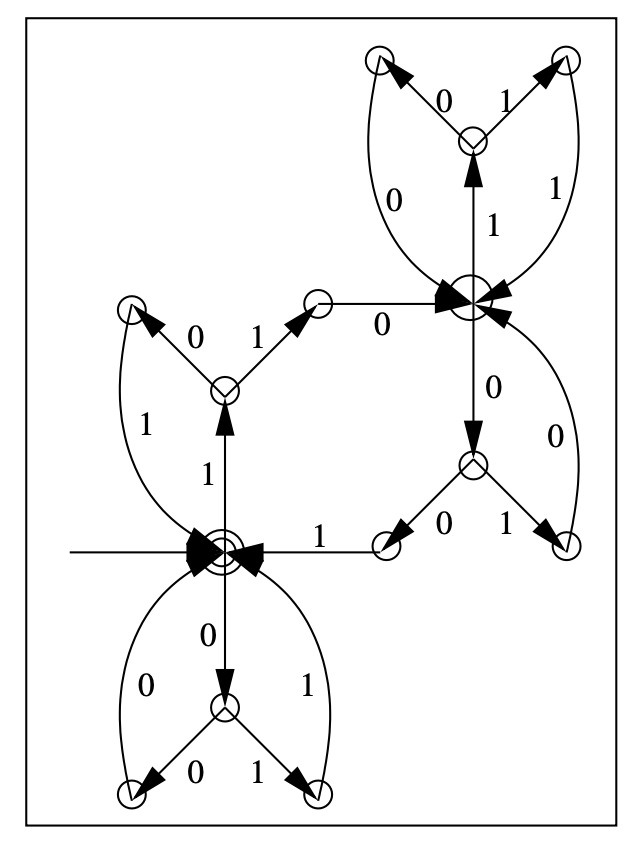
\includegraphics[scale = 0.35]{Images/Optelchecker.png}
    \end{minipage}
\end{theo}